\documentclass[11pt]{amsart}
\usepackage[margin=1in]{geometry}
\usepackage{amsmath,amssymb,amsthm,mathtools,booktabs,enumitem,xcolor,graphicx,hyperref}
\hypersetup{colorlinks=true,linkcolor=blue!50!black,citecolor=blue!50!black,urlcolor=blue!50!black}

\newtheorem{theorem}{Theorem}[section]
\newtheorem{lemma}[theorem]{Lemma}
\newtheorem{proposition}[theorem]{Proposition}
\newtheorem{corollary}[theorem]{Corollary}
\theoremstyle{definition}
\newtheorem{definition}[theorem]{Definition}
\newtheorem{remark}[theorem]{Remark}

\newcommand{\R}{\mathbb{R}}
\newcommand{\Q}{\mathbb{Q}}
\newcommand{\sq}{\sqrt5}
\newcommand{\gr}{\varphi}          % golden ratio
\newcommand{\Prj}{\Pi}
\newcommand{\ip}[2]{\langle #1,#2\rangle}
\newcommand{\abs}[1]{\lvert #1\rvert}
\newcommand{\norm}[1]{\lVert #1\rVert}
\newcommand{\RID}{\mathcal{P}}
\newcommand{\Ih}{I_h}

\title{The rhombicosidodecahedron is not Rupert}
\author{Gihyo Jung}
\address{Independent researcher, Republic of Korea}
\email{swiri0921@gmail.com}
\date{October 2026}

\begin{document}
\begin{abstract}
A convex body is \emph{Rupert} if a hole can be cut through it such that a congruent copy can pass through the hole.
Steininger and Yurkevich recently constructed the first convex polyhedron without this property; earlier they had
conjectured that the rhombicosidodecahedron is not Rupert either. We prove this conjecture by a computer-assisted proof.
The subdivision method of Steininger and Yurkevich does not suffice for the rhombicosidodecahedron on its own:
because of its large symmetry group there are one-parameter families of configurations in which the two shadows
coincide, and at four exceptional configurations the first-order protection that the method relies on degenerates.
We describe these coincidences, locate the four singular configurations exactly in $\Q(\sq)$, and prove three new
local certificates: a fixed-direction coincidence theorem, a multi-contact gradient theorem and a blow-up
(sector and arc-tube) theorem at singular points. All inequalities of the certificates are verified in outward-rounded
interval arithmetic, and all structural identities are verified in exact arithmetic in $\Q(\sq)$.
\end{abstract}

\maketitle


%==========================================================================================
\section{Introduction}\label{sec:intro}

According to John Wallis (1693), Prince Rupert of the Rhine wagered that a hole can be cut in a cube through which a
cube of the same size can pass. A convex body $K\subset\R^3$ is called \emph{Rupert} if there are rotations $O_1,O_2\in SO(3)$ and
a vector $t\in\R^2$ such that
\begin{equation}\label{eq:rupert}
  \Prj O_1 K + t \subset \operatorname{int}\bigl(\Prj O_2 K\bigr),
\end{equation}
where $\Prj:\R^3\to\R^2$ is the orthogonal projection $(x,y,z)\mapsto(x,y)$. All five Platonic solids and many
Archimedean and Catalan solids are Rupert \cite{JWY17,Chai18,Hoff19,Lav22,Fre21}. Steininger and Yurkevich \cite{SY25}
constructed the first convex polyhedron that is not Rupert (the \emph{Noperthedron}). Earlier, in \cite{SY21},
they proved that the truncated icosidodecahedron is Rupert, so that ten of the thirteen Archimedean solids are known
to be Rupert, and conjectured on statistical evidence that the rhombicosidodecahedron is not \cite[Conjecture 2]{SY21};
the snub cube and the snub dodecahedron remain open.
Extensive numerical searches \cite{SY21,Gos25} found no passage for the rhombicosidodecahedron. (For computational
evidence that a certain stellated tetrahedron is not Rupert, see \cite{Zeng26}.)

\begin{theorem}\label{thm:main}
The rhombicosidodecahedron is not Rupert.
\end{theorem}

\subsection*{Method and difficulties}
Steininger and Yurkevich \cite{SY25} parametrise the pairs of projections by a five-dimensional box, subdivide it,
and exclude every sub-box either by a \emph{global theorem} (a separating direction that works on the whole box) or by
a \emph{local theorem} near configurations in which the two shadows coincide. For the Noperthedron, which was
designed to have a small symmetry group, these two tools suffice. In \cite[Section 9.1]{SY25} the authors explain
that for the rhombicosidodecahedron their local theorem cannot be applied at the view along a coordinate axis of the
standard coordinates (a two-fold axis; this is our point $A$ below) and in about $2\%$ of random view directions. For the rhombicosidodecahedron $\RID$ (symmetry group
$\Ih$ of order 120) they do not, for three reasons which we identify in Section~\ref{sec:coinc}:
\begin{enumerate}[label=(\roman*)]
\item there are many more coincidences: the shadows coincide whenever $O_1=D\,O_2\,g$ with $g$ in the rotation group
  $I$ and $D\in\{I,\rho_\pi\}$ ($\rho_\pi$ the half-turn about the viewing axis); in the reduced parameter domain two
  such branches cross at views along a two-fold axis; and on an arc of \emph{half-twist} configurations, in which the
  inner body is the outer one rotated by $36^\circ$ about a five-fold axis, the inner shadow touches the outer one
  from inside;
\item at a view along a two-fold axis and at a view orthogonal to a five-fold axis (points $A$, $B$) the linear
  protection of the local theorem degenerates: the protrusion of the inner shadow is only of order
  $\abs{w}\,\abs{\xi}$, where $w$ is the offset of the view and $\xi$ the relative rotation;
\item at the two endpoints $C$, $D$ of the half-twist arc the protection degenerates in a different way (the
  protrusion vanishes identically along a curve).
\end{enumerate}
Near the coincidences of (i), boxes are closed by the local theorem of \cite{SY25}, whose orthogonal map need not be a
symmetry of the polyhedron (this closes the interior of the half-twist arc), and by a fixed-direction version of the
local theorem (Theorem~\ref{thm:local2}); a multi-contact gradient certificate (Theorem~\ref{thm:local5}) closes boxes
close to, but not containing, coincidences. We deal with (ii), (iii) by blow-up certificates (Theorems~\ref{thm:sector} and~\ref{thm:tube}) that are valid in a whole neighbourhood of the
singular configuration, including the singular configuration itself.

\subsection*{Rigour}
All inequalities of the certificates are checked in outward-rounded interval arithmetic (Section~\ref{sec:ia}); the few
combinatorial decisions taken in floating point, all with large slack, are listed in Appendix~\ref{app:float}. All
statements of the form ``this quantity is exactly zero'' (collinearity of projected vertices at a singular view,
identical vertex trajectories, exactness of a contact along the half-twist arc, a vertex lying in the shadow plane)
are proved in exact arithmetic in $\Q(\sq)$, using exact coordinates of the singular configurations
(Proposition~\ref{prop:exact}). The code and the certificates are available at \url{https://github.com/swiri0921-bit/rhombicosidodecahedron-not-rupert}
(release \texttt{v1.1}; the file \texttt{results/CODE\_HISTORY.md} lists the hashes of the programs used for the runs).

\subsection*{Use of AI}
The author chose the problem, planned and directed the project, and made the decisions on how to proceed at each
stage. In particular, the author proposed to write out and audit the hand proofs of all certificates while the
computations were running; this audit led to the detection and correction of several errors before the final run.
The author ran a large part of the computations on his own computer, monitored them to completion, and prepared the
public repository. An AI system (Claude, by Anthropic) was used extensively as a research assistant: for the
literature search, for developing the mathematical arguments and the programs, for running computations, and for
drafting the text; the second and third implementations used for the checks of Section~\ref{sec:indep} were written with the same
assistance. The proof does not ask the reader to trust the AI system: all statements are proved in this paper, and
every computer-verified statement can be reproduced and checked with the published programs and result files.

%==========================================================================================
\section{Setup}\label{sec:setup}

\subsection{The polyhedron}
Let $\gr=(1+\sq)/2$. The rhombicosidodecahedron $\RID$ is the convex hull of the $60$ points obtained from
\[
(\pm1,\pm1,\pm\gr^3),\qquad (\pm\gr^2,\pm\gr,\pm2\gr),\qquad (\pm(2+\gr),0,\pm\gr^2)
\]
by cyclic permutations of the coordinates. We rotate $\RID$ so that the five-fold axis through $(0,\gr,1)$ becomes the
$z$-axis and scale it to circumradius $1$; we denote its vertices by $V_1,\dots,V_{60}$, $\abs{V_k}=1$. The rotation is
not rational; wherever exact values are needed we work in the body frame (coordinates in $\Q(\sq)$), and the rotated
coordinates are enclosed in intervals computed from decimal values with error below $10^{-55}$ (Section~\ref{sec:ia}). $\RID$ is
centrally symmetric: $-V_k=V_{k'}$.

\subsection{Parametrisation}
Following \cite{SY25}, for $\theta,\phi\in\R$ let
\[
M(\theta,\phi)=\begin{pmatrix}-\sin\theta&\cos\theta&0\\-\cos\theta\cos\phi&-\sin\theta\cos\phi&\sin\phi\end{pmatrix},
\qquad X(\theta,\phi)=(\cos\theta\sin\phi,\ \sin\theta\sin\phi,\ \cos\phi),
\]
so that $M(\theta,\phi)$ is the projection along the view direction $X(\theta,\phi)$, and let $R(\alpha)$ be the
rotation of $\R^2$ by $\alpha$. We write $A(\theta,\phi)\in SO(3)$ for the matrix with rows the two rows of $M$ and
$X$. Every $O\in SO(3)$ satisfies $\Prj O = R(\alpha)M(\theta,\phi)$ for suitable $(\theta,\phi,\alpha)$.

\begin{lemma}[reductions]\label{lem:reduce}
If $\RID$ is Rupert, then there is $x=(\theta_1,\phi_1,\theta_2,\phi_2,\alpha)$ in
\[
\mathcal{D}=[0,2\pi/5]\times[0,\phi_{\max}]\times[0,2\pi/5]\times[0,\phi_{\max}]\times[-\pi/2,\pi/2],
\qquad \phi_{\max}=0.6524,
\]
with $R(\alpha)M(\theta_1,\phi_1)\RID\subset\operatorname{int} M(\theta_2,\phi_2)\RID$ (no translation).
\end{lemma}
\begin{proof}
\emph{Translation.} If $S+t\subset\operatorname{int}T$ for centrally symmetric convex sets $S,T$, then also
$S-t=-(S+t)\subset\operatorname{int}T$, and by convexity $S\subset\operatorname{int}T$ (see \cite{SY25}).
\emph{Symmetries.} Replacing $O_i$ by $O_i g_i$ with $g_i$ in the rotation group $I\subset\Ih$ does not change the
bodies $O_i\RID$. The view direction of $O_i$ is $O_i^{T}e_3$, and every unit vector is within the angle
$\arccos\sqrt{(5+2\sq)/15}=0.652358\ldots<\phi_{\max}$ (about $37.38^\circ$) of one of the twelve five-fold axes (this is the angle between a
five-fold and an adjacent three-fold axis, the covering radius of the five-fold axes), so we may assume that both view
directions are within $\phi_{\max}$ of $e_3$. Since $M(\theta+2\pi/5,\phi)=M(\theta,\phi)R_z(-2\pi/5)$ and
$R_z(2\pi/5)\in I$, $\theta_i\in[0,2\pi/5]$. Finally $R(\alpha+\pi)=-R(\alpha)$ and $\RID=-\RID$, so
$\alpha\in[-\pi/2,\pi/2]$. The outer rotation about the view axis can be absorbed into $\alpha$.
\end{proof}

We call $x\in\mathcal D$ a \emph{passage} if $R(\alpha)M(\theta_1,\phi_1)\RID\subset\operatorname{int}M(\theta_2,\phi_2)\RID$.
Theorem~\ref{thm:main} is equivalent to: \emph{$\mathcal{D}$ contains no passage}. To exclude a set of
configurations it suffices to exhibit, for each $x$, a direction $n\in\R^2\setminus\{0\}$ and an inner vertex $i$ with
\begin{equation}\label{eq:protrusion}
  P_{i,n}(x):=\ip{p_i(x)}{n}-\max_k\ip{q_k(x)}{n}\ \ge\ 0,\qquad p_i=R(\alpha)M(\theta_1,\phi_1)V_i,\ \ q_k=M(\theta_2,\phi_2)V_k .
\end{equation}
Indeed, $P_{i,n}\ge0$ says that $p_i$ is not in the interior of the outer shadow.

\subsection{Derivative bounds}
All maps below are products of rotations about fixed axes, each depending on one parameter at unit speed.
\begin{lemma}\label{lem:deriv}
Let $R_3(\theta)$ be the rotation about $e_3$ by $\theta$. Then $A(\theta,\phi)=B(\phi)R_3(\theta)^T$, where the rows of
$B(\phi)$ are $e_2$, $-\cos\phi\,e_1+\sin\phi\,e_3$ and $\sin\phi\,e_1+\cos\phi\,e_3$. Consequently
\[
\partial_\theta A=A\,S_\theta,\qquad \partial_\phi A=S_\phi A,\qquad \partial_\alpha\operatorname{diag}(R(\alpha),1)=S_\alpha\operatorname{diag}(R(\alpha),1)
\]
with constant skew matrices $S_\theta,S_\phi,S_\alpha$ of operator norm $1$. Hence all first and second partial
derivatives of $A$, of $A_{\rm in}=\operatorname{diag}(R(\alpha),1)A(\theta_1,\phi_1)$ and of their products with fixed
rotations have operator norm at most $1$, and:
\begin{enumerate}[label=(\alph*)]
\item $\norm{A(\theta,\phi)-A(\theta_0,\phi_0)}\le\abs{\theta-\theta_0}+\abs{\phi-\phi_0}$;
\item the rotation angles of $A_{\rm in}(x)A_{\rm in}(x_0)^T$ and of $A_{\rm out}(x)A_{\rm out}(x_0)^T$ are at most
 $\sum_{d\in\{1,2,5\}}\abs{x_d-x_d^0}$ and $\abs{x_3-x_3^0}+\abs{x_4-x_4^0}$, respectively;
\item for $\abs V\le1$ and $n\in\R^2$ the functions $x\mapsto\ip{\Prj A_{\rm in}(x)V}{n}$, $\ip{\Prj A_{\rm out}(x)V}{n}$ differ
 from their first-order Taylor polynomials at $x_0$ by at most $\tfrac12\bigl(\sum_d\abs{x_d-x_d^0}\bigr)^2\abs n$, where
 $d$ ranges over $\{1,2,5\}$ for the inner and over $\{3,4\}$ for the outer body.
\end{enumerate}
\end{lemma}
\begin{proof}
The factorisation is checked directly from the definition of $M$ and $X$. Since
$\partial_\theta R_3(\theta)^T=R_3(\theta)^T[e_3]^T$, we get
$\partial_\theta A=A\,[e_3]^T$, a constant skew matrix of norm $1$; $B'(\phi)$ rotates the second and third rows
into each other, $B'=S_\phi B$. Second derivatives are products of a rotation and two such generators, and
$\norm{S^2}\le1$. (a) and (c) follow from the mean value theorem and Taylor's theorem. For (b), the angle of $Q\in SO(3)$
is its distance to $I$ in the bi-invariant metric, and $t\mapsto A_{\rm in}(x_0+t(x-x_0))$ has angular speed at most
$\sum_d\abs{x_d-x_d^0}$.
\end{proof}

%==========================================================================================
\section{Coincidences and singular configurations}\label{sec:coinc}

\subsection{Coincidences}
A configuration $x$ is a \emph{coincidence} if the two shadows are equal. Coincidences are never passages, but no
box containing a coincidence can be excluded by a separating-direction argument, so every coincidence must be dealt
with by a local theorem. Writing the inner orientation as
$A_{\rm in}=e^{[\xi]}\,D\,A_{\rm out}\,h$ with $\xi\in\R^3$ (rotation vector, $[\xi]$ the cross-product matrix), the
following configurations have to be treated as coincidences.
\begin{enumerate}[label=(\alph*)]
\item \emph{Symmetry coincidences}: $\xi=0$, $h\in I$ and $D\in\{I,\rho_\pi\}$, $\rho_\pi=\operatorname{diag}(-1,-1,1)$
  (rotation by $\pi$ about the viewing axis; $\Prj\rho_\pi=-\Prj$ and $\RID=-\RID$). In the reduced domain
  $\mathcal D$ these form several branches. Two of them meet at views along a two-fold axis $a$: if $h_a\in I$ is the
  half-turn about $a$ and $X=a$, then $A_{\rm out}h_aA_{\rm out}^T=\rho_\pi$, so the branches $A_{\rm in}=A_{\rm out}$ and
  $A_{\rm in}=\rho_\pi A_{\rm out}h_a$ coincide there, while for views near $a$ they differ by a small rotation
  (Lemma~\ref{lem:psi}).
\item \emph{Half-twist configurations}: $A_{\rm in}=A_{\rm out}T$ with $T$ the rotation by $36^\circ$ about the
  five-fold axis $a=(\gr,1,0)$ (body frame) composed with an element of $I$ (the exact matrices $T_C,T_D$ are given in
  the repository). The axis $a$ and the five-fold axis $w_5=(0,\gr,1)$ of the viewing cap span a mirror plane and
  enclose the angle $\arctan2$. The twenty vertices of the two decagonal rings orthogonal to $a$ are mapped to
  vertices, and for outer views $X$ in this mirror plane, between $w_5$ and $a$, with
  $\angle(X,w_5)\in[\arctan\gr^{-5},\ \arctan\tfrac13]$ (so that $\angle(X,a)=\arctan2-\angle(X,w_5)$ lies between
  $45^\circ$ and about $58.3^\circ$) the inner shadow lies in the outer one and shares boundary
  points with it (Figure~\ref{fig:shadowsC}). On this \emph{half-twist arc} the protrusion is exactly $0$ (so these
  configurations are not passages); the arc is not a family of coincidences in the strict sense, but it has to be
  treated like one. Near interior points of the arc, three inner and three outer vertices of the relevant contacts are
  congruent via an orthogonal map which is not a symmetry of $\RID$; boxes there are closed by the local theorem of
  \cite{SY25} (Section~\ref{sec:cert}).
\end{enumerate}
This description guides the choice of certificates, but the proof does not depend on its completeness: every box of
$\mathcal D$ is closed by one of the certificates of Section~\ref{sec:cert}.

\subsection{Singular configurations}
Near a symmetry coincidence $x_0$ with outer view $X_0$ the protrusion is, to first order,
$\max_c\ip{\xi}{g_c}$ where $g_c = U_i\times N$ ranges over the contacts (Theorem~\ref{thm:local2}). If the cone
spanned by the $g_c$ is all of $\R^3$, a whole neighbourhood of $x_0$ is excluded. This fails exactly at views where
several faces are seen edge-on. A numerical scan of the cap finds six views with at least two edge-on faces; at four
of them the protection vanishes (Table~\ref{tab:sing}). (The scan is not part of the proof; its role is to locate the
points where blow-up certificates are needed.)

\begin{proposition}[exact singular configurations]\label{prop:exact}
In the body frame (coordinates as in Section~\ref{sec:setup}, up to scale) the singular views are
\[
X_A=(1,\gr,\gr-1),\quad X_B=\bigl(1,\tfrac{5+\sq}{2},\tfrac{\sq-1}{2}\bigr),\quad
X_C=\bigl(1,\tfrac{9+5\sq}{2},\tfrac{5+3\sq}{2}\bigr),\quad X_D=\bigl(1,\tfrac{3\sq-1}{2},\tfrac{5-\sq}{2}\bigr).
\]
The half-twist rotations $T_C,T_D$ have entries in $\Q(\sq)$ in the body frame. (Geometrically, $X_A$ is a two-fold
axis, $X_B$ is orthogonal to a five-fold axis in a mirror plane, and $X_C$, $X_D$ are the endpoints of the half-twist
arc; these descriptions, checked numerically, are for orientation only: the proof uses only the exact coordinates.)
\end{proposition}
\begin{proof}
The coordinates are exact elements of $\Q(\sq)^3$; all identities used in the certificates are verified in exact
arithmetic (file \texttt{exact\_check.py}, Section~\ref{sec:exactid}). For $T$: the rotation by $36^\circ$
about $a=(\gr,1,0)$ is $\cos36^\circ I+\sin36^\circ[\hat a]+(1-\cos36^\circ)\hat a\hat a^{T}$ with $\cos36^\circ=\gr/2$
and $\sin 36^\circ/\abs{a}=(\sq-1)/4$, so all entries lie in $\Q(\sq)$.
\end{proof}

\begin{figure}[h]
\centering
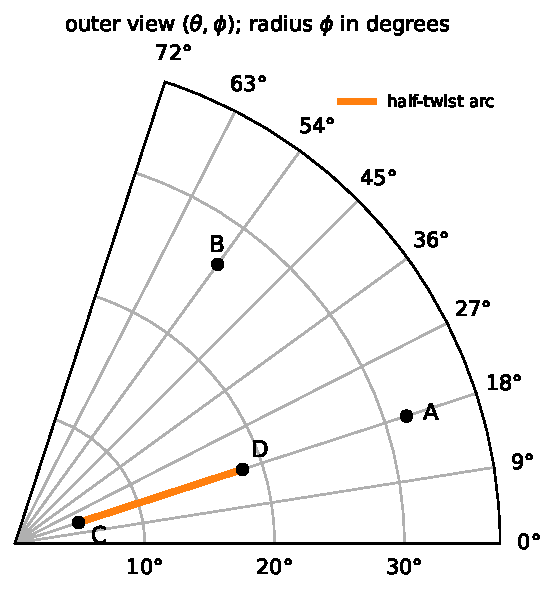
\includegraphics[width=0.42\textwidth]{fig/cap.pdf}
\caption{The reduced range of outer views ($\theta\in[0,72^\circ]$, $\phi\le37.38^\circ$) with the singular views $A,B,C,D$ and
the half-twist arc from $C$ ($\phi=\arctan\gr^{-5}$) to $D$ ($\phi=\arctan\frac13$).}\label{fig:cap}
\end{figure}
\begin{figure}[h]
\centering
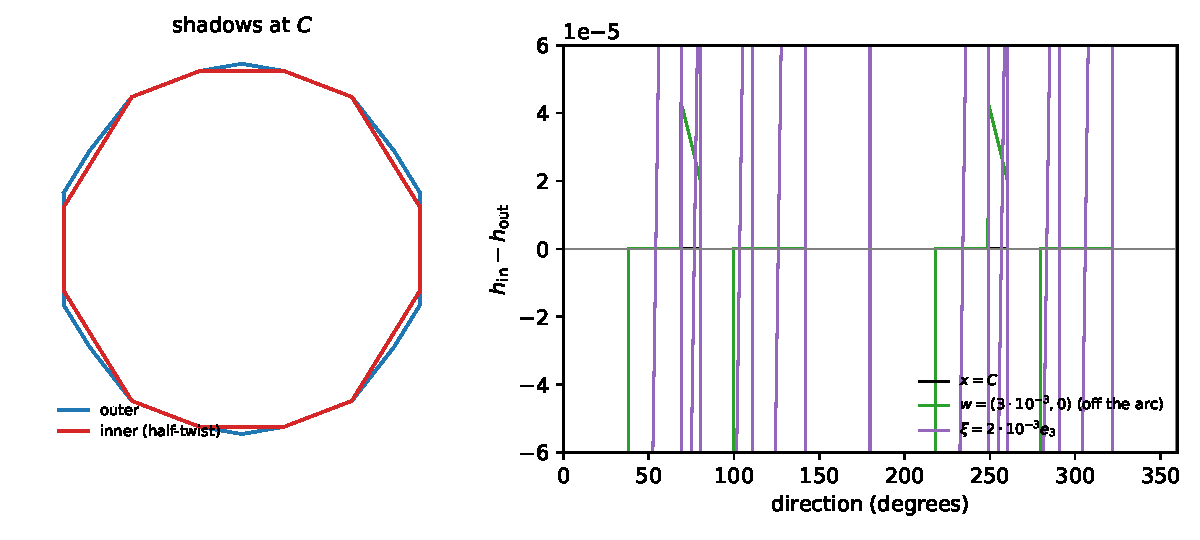
\includegraphics[width=0.95\textwidth]{fig/shadowsC.pdf}
\caption{Left: outer shadow and half-twisted inner shadow at $C$. Right: $h_{\rm in}-h_{\rm out}$ (difference of support
functions) as a function of the direction; at $C$ its maximum is exactly $0$ on whole intervals of directions, off the
arc or after a small rotation it becomes positive. The vertical scale is $10^{-5}$.}\label{fig:shadowsC}
\end{figure}

\begin{table}[h]
\centering\small
\begin{tabular}{@{}lllll@{}}
\toprule
point & view & coincidence type & degeneracy & treatment\\ \midrule
$A$ & two-fold axis & two symmetry branches & $P\sim c\,\abs{w}\abs{\xi}$ & sector, two references\\
$B$ & $\perp$ five-fold axis & symmetry & $P\sim c\,\abs{w}\abs{\xi}$ & sector\\
$C$ & arc endpoint & half-twist (two branches) & $P\equiv0$ on the arc & two arc tubes + sector ($s$-mode)\\
$D$ & arc endpoint & half-twist & $P\equiv0$ on the arc & arc tube + sector ($s$-mode)\\ \bottomrule
\end{tabular}
\caption{The four singular configurations.}\label{tab:sing}
\end{table}

%==========================================================================================
\section{Certificates}\label{sec:cert}

We use six certificates. Each takes a box $\mathcal B\subset\mathcal D$ (or a region in blow-up coordinates) and some
floating-point data (a direction, multipliers of a linear program), and each has a conclusion of the form
``$\mathcal B$ contains no passage'' whose hypotheses are finitely many inequalities verified in interval arithmetic
and finitely many identities verified in $\Q(\sq)$. Floating-point data are only \emph{witnesses}: they are never
assumed to be exact.

\subsection{The theorems of Steininger and Yurkevich}
We use the global theorem \cite[Theorem 17]{SY25} and the local theorem \cite[Theorem 36]{SY25} in the form stated
there (with $\rho=1$ and $\varepsilon$ the largest half-width of the box, rounded upward; the theorems then apply to a cube
containing the box). The local theorem requires two triples of vertices to be
\emph{congruent}, i.e.\ related by an orthonormal matrix $L$ \cite[Definition 34]{SY25}; $L$ need not be a symmetry of
the polyhedron, and near the interior of the half-twist arc it is not. We certify congruence either by a symmetry
of $\RID$ mapping one triple to the other, or by checking that the Gram matrices of the two triples are equal in
$\Q(\sq)$, which is equivalent to the existence of such an $L$ (possibly with determinant $-1$). The inequalities
checked for the local theorem are listed in Appendix~\ref{app:sylocal}.

\subsection{Fixed-direction coincidence theorem}
\begin{theorem}\label{thm:local2}
Let $\mathcal B$ be a box with centre $x_0$ and largest half-width $\varepsilon$. Let $h\in I$ and $D\in\{I,\rho_\pi\}$, and put
$U_i(x)=D A_{\rm out}(x)hV_i$ and $e^{[\xi(x)]}=A_{\rm in}(x)\bigl(DA_{\rm out}(x)h\bigr)^{T}$, so that the inner body is
$\{e^{[\xi]}U_i\}$ and $\Prj U_i=\Prj A_{\rm out}V_{k(i)}$ for a bijection $k$. Let $n_1,\dots,n_m$ be unit vectors in
$\R^2$ and $k_c$ vertices such that for every $c$ and every $x\in\mathcal B$, $k_c$ is the unique maximiser of
$\ip{\Prj A_{\rm out}(x)V_j}{n_c}$. Let $g_c=U_{i_c}(x_0)\times N_c$ with $N_c=(n_c,0)$ and $i_c=k^{-1}(k_c)$, and
\[
c_0=\min_{\abs v=1}\max_c\ \ip{v}{g_c},\qquad \xi_{\max}=\abs{\xi(x_0)}+5\varepsilon .
\]
If $c_0-2\varepsilon>\xi_{\max}/2+\xi_{\max}^2/6$, then $\mathcal B$ contains no passage.
\end{theorem}
\begin{proof}
Fix $x\in\mathcal B$ and write $\xi=\xi(x)$, $U_i=U_i(x)$. If $\xi=0$ the shadows coincide and $x$ is not a
passage. Otherwise, since $k_c$ is the unique maximiser and $\Prj U_{i_c}=\Prj A_{\rm out}V_{k_c}$,
\[
P_{i_c,n_c}(x)=\ip{\Prj(e^{[\xi]}-I)U_{i_c}}{n_c}=\ip{(e^{[\xi]}-I)U_{i_c}}{N_c}.
\]
For a rotation by angle $\vartheta=\abs\xi$ one has
$\norm{e^{[\xi]}-I-[\xi]}=\norm{(1-\cos\vartheta)[\hat\xi]^2+(\sin\vartheta-\vartheta)[\hat\xi]}\le\vartheta^2/2+\vartheta^3/6$,
hence, with $\abs{U_i}=1$, $P_{i_c,n_c}\ge\ip{\xi}{U_{i_c}\times N_c}-\abs\xi^2/2-\abs\xi^3/6$.
By Lemma~\ref{lem:deriv}, $\abs{U_i(x)-U_i(x_0)}\le2\varepsilon$, so $\ip{\xi}{U_{i_c}(x)\times N_c}\ge\abs\xi(\ip{\hat\xi}{g_c}-2\varepsilon)$,
and the angle of $e^{[\xi(x)]}$ is at most $\abs{\xi(x_0)}+3\varepsilon+2\varepsilon$. Choosing $c$ with
$\ip{\hat\xi}{g_c}\ge c_0$ gives $P_{i_c,n_c}(x)\ge\abs\xi\,(c_0-2\varepsilon-\xi_{\max}/2-\xi_{\max}^2/6)>0$.
\end{proof}
\noindent\emph{Verification.} The directions $n_c$ are interior directions of the normal cones of the outer shadow at
$x_0$; unique maximality on $\mathcal B$ is checked by $\ip{\Prj A_{\rm out}(x_0)(V_{k_c}-V_j)}{n_c}>2\varepsilon\abs{V_{k_c}-V_j}$
for all $j\ne k_c$ (Lemma~\ref{lem:deriv}). The rotation angle of $e^{[\xi(x_0)]}$ is bounded from
$y=\norm{e^{[\xi]}-I}_F/\sqrt8=\sin(\vartheta/2)$ by $\vartheta\le 2y/\sqrt{1-y^2}$. The number $c_0$ is bounded below by
covering the sphere by caps of radius $r=1.001\cdot\sqrt2/48$ around the normalised centres of the cells of a
$48\times48$ grid on each face of the cube $[-1,1]^3$ (radial projection onto the sphere is $1$-Lipschitz on the cube surface) and using
$\ip{v}{g}\ge\ip{p}{g}-r\abs g$. The symmetry $h$ is enclosed from $60$-digit data of the exact matrix.

\subsection{Multi-contact gradient certificate}
\begin{theorem}\label{thm:local5}
Let $\mathcal B$ be a box with centre $x_0$ and half-widths $\delta^{\max}\in\R^5$. Let $(i_c,n_c,K_c)_{c=1}^m$ be
contacts (inner vertex, direction, set of outer vertices) and $\lambda\in\R^m_{\ge0}\setminus\{0\}$. Suppose
\begin{enumerate}[label=(\alph*)]
\item for every $c$, every $j\notin K_c$: $\sup_{\mathcal B}\ip{q_j}{n_c}\le\max_{k\in K_c}\inf_{\mathcal B}\ip{q_k}{n_c}$
 (bounds from first-order Taylor expansion plus the remainder of Lemma~\ref{lem:deriv});
\item at each of the $32$ vertices $\delta$ of $\prod_d[-\delta^{\max}_d,\delta^{\max}_d]$,
\[
\sum_c\lambda_c\Bigl(\ell_{i_c}(\delta)-\max_{k\in K_c}\ell_{k}(\delta)-\tfrac12\bigl(h_{\rm in}^2+h_{\rm out}^2\bigr)\abs{n_c}\Bigr)>0,
\]
where $\ell_i$, $\ell_k$ are the first-order Taylor polynomials at $x_0$ of $\ip{p_i}{n_c}$ and $\ip{q_k}{n_c}$, and
$h_{\rm in}=\delta^{\max}_1+\delta^{\max}_2+\delta^{\max}_5$, $h_{\rm out}=\delta^{\max}_3+\delta^{\max}_4$.
\end{enumerate}
Then $\mathcal B$ contains no passage.
\end{theorem}
\begin{proof}
By (a) the maximum in \eqref{eq:protrusion} is attained in $K_c$. By Lemma~\ref{lem:deriv},
$P_{i_c,n_c}(x_0+\delta)\ge F_c(\delta):=\ell_{i_c}(\delta)-\max_{k\in K_c}\ell_k(\delta)-\tfrac12(h_{\rm in}^2+h_{\rm out}^2)\abs{n_c}$.
The function $\sum_c\lambda_cF_c$ is concave (a sum of minima of affine functions), so its minimum over the box is
attained at a vertex, where it is positive by (b). Hence some $P_{i_c,n_c}(x)>0$ for every $x\in\mathcal B$.
\end{proof}

\subsection{Blow-up coordinates at a singular point}
Let $x^*$ be one of $A,B,C,D$ with outer view $(\theta^*,\phi^*)$, and fix a \emph{reference} $A_{\rm ref}(w)=M_{\rm f}A(w)T$
for the inner body, where $A(w)=A(\theta^*+w_1,\phi^*+w_2)$, $T$ is a fixed rotation ($T\in I$ at $A,B$: $T=I$, and $T=h$ for the
second reference $\rho_\pi A(w)h$ at $A$; a half-twist at $C,D$), and $M_{\rm f}\in\{I,\rho_\pi\}$. Every configuration near $x^*$ is
written as
\[
A_{\rm out}=A(w),\qquad A_{\rm in}=e^{[\xi]}A_{\rm ref}(w),\qquad (w,\xi)\in\R^2\times\R^3 .
\]
Put $U_i(w)=A_{\rm ref}(w)V_i$, $W_k(w)=A(w)V_k$ and $s=\max(\abs w,\abs\xi)$; for $s>0$ write $w=s\hat w$, $\xi=s\tau\omega$
with $\abs\omega=1$, $\tau\in[0,1]$. Since $\Prj\rho_\pi=-\Prj$ we have $\Prj(W_k-U_i)(w)=\Prj A(w)d_{ik}$ with the fixed vector
$d_{ik}=V_k-\sigma TV_i$, $\sigma=\pm1$ according to $M_{\rm f}$.

For a line $j$ of the outer shadow at $x^*$ (the projection of an edge, or a supporting line at a vertex) with outer unit
normal $n_j$ and level $H_j$ let $K_j=\{k:\ip{\Prj W_k(0)}{n_j}=H_j\}$ and $I_j=\{i:\ip{\Prj U_i(0)}{n_j}=H_j\}$; these
sets are certified exactly (Section~\ref{sec:exactid}). A \emph{contact} is $c=(i,j,\phi,\chi)$ with $i\in I_j$ and
direction $n_c=R(s\phi+\chi w_1)n_j$; $N_c=(n_c,0)$. Its protrusion is
$P_c=\ip{\Prj e^{[\xi]}U_i}{n_c}-\max_k\ip{\Prj W_k}{n_c}$.

\begin{lemma}[second-order rotation formula]\label{lem:rot}
For $\xi=\vartheta\omega$ ($\abs\omega=1$) and vectors $U,N$,
\[
\ip{e^{[\xi]}U}{N}=\ip UN+\ip{\xi}{U\times N}+\tfrac12\abs\xi^2\,q(\omega)+R,\qquad
q(\omega)=\ip\omega U\ip\omega N-\ip UN,
\]
with $\abs R\le\bigl(\vartheta^3/6+\vartheta^4/24\bigr)\abs U\abs N$.
\end{lemma}
\begin{proof}
Rodrigues' formula $e^{[\xi]}=I+\sin\vartheta[\omega]+(1-\cos\vartheta)[\omega]^2$, $[\omega]U=\omega\times U$,
$\ip{[\omega]^2U}{N}=q(\omega)$, and $\abs{\sin\vartheta-\vartheta}\le\vartheta^3/6$,
$\abs{1-\cos\vartheta-\vartheta^2/2}\le\vartheta^4/24$, $\norm{[\omega]}=\norm{[\omega]^2}=1$.
\end{proof}

\begin{lemma}[contact expansion]\label{lem:contact}
Fix a contact $c=(i,j,\phi,\chi)$, $\hat w$ and $\omega$, and let
\[
g_0=U_i(0)\times N_j,\qquad b(\hat w)=\tfrac{d}{ds}\big|_{s=0}\,U_i(s\hat w)\times N_c,\qquad
\alpha_k(\hat w)=\tfrac{d}{ds}\big|_{s=0}\ip{\Prj(W_k-U_i)(s\hat w)}{n_c},
\]
$f=\abs{\hat w}_1+\abs\phi+\abs\chi\abs{\hat w_1}$ and $q_0=q(\omega)$ computed with $U=U_i(0)$, $N=N_j$. Then for
$k\in K_j$ and $\vartheta=\abs\xi$,
\begin{multline*}
\ip{\Prj e^{[\xi]}U_i}{n_c}-\ip{\Prj W_k}{n_c}\ \ge\ \vartheta\Bigl(\ip\omega{g_0}+s\ip\omega b-\tfrac12f^2s^2\Bigr)
+\tfrac12\vartheta^2q_0-\tfrac12\vartheta^2fs-\Bigl(\frac{\vartheta^3}6+\frac{\vartheta^4}{24}\Bigr)\\
-s\,\alpha_k-\tfrac12\abs{d_{ik}}f^2s^2 .
\end{multline*}
\end{lemma}
\begin{proof}
Write the left side as $\ip{(e^{[\xi]}-I)U_i}{N_c}+\ip{\Prj(U_i-W_k)}{n_c}$ and apply Lemma~\ref{lem:rot} with
$U=U_i(s\hat w)$, $N=N_c(s)$, $\abs U=\abs N=1$. Along $s\mapsto s\hat w$ the frame $A(s\hat w)$ has derivatives of norm
$\le\abs{\hat w}_1$ and second derivatives of norm $\le\abs{\hat w}_1^2$ (Lemma~\ref{lem:deriv}), and $n_c$ rotates at
speed $\abs{\phi+\chi\hat w_1}\le\abs\phi+\abs\chi\abs{\hat w_1}$. Hence $\abs{\frac{d^2}{ds^2}(U\times N)}\le f^2$, which
gives the first bracket. For $q$ note $\frac{d}{ds}q=-\ip{U'}{N-\omega\ip\omega N}-\ip{N'}{U-\omega\ip\omega U}$, so
$\abs{\frac{d}{ds}q}\le\abs{U'}+\abs{N'}\le f$. Finally $s\mapsto\ip{\Prj A(s\hat w)d_{ik}}{n_c(s)}$ vanishes at $0$ (as
$i\in I_j$, $k\in K_j$), has derivative $\alpha_k$ at $0$ and second derivative bounded by $\abs{d_{ik}}f^2$.
\end{proof}

\begin{lemma}[inactive vertices]\label{lem:inactive}
For a contact $c=(i,j,\phi,\chi)$ let
\[\Delta_j=\min_{k\notin K_j}\bigl(H_j-\ip{\Prj W_k(0)}{n_j}\bigr)>0\]
and let
\[
a_k=\max\Bigl(\abs{\partial_{w_1}\ip{\Prj(W_k-U_i)}{n_j}}+\abs{\partial_{w_2}\ip{\Prj(W_k-U_i)}{n_j}},\ \abs{\ip{\Prj(W_k-U_i)(0)}{n_j^{\perp}}}\Bigr)
\]
at $w=0$, $a_{\rm in}=\max_{k\notin K_j}a_k$, $a_{\rm act}=\max_{k\in K_j}a_k$. If
\[
r_0\,(a_{\rm in}+a_{\rm act})\,(1+\abs\phi+\abs\chi)+4r_0^2\bigl(\sqrt2+\abs\phi+\abs\chi\bigr)^2<\Delta_j ,
\]
then for $\abs{\hat w}_\infty\le1$ and $0<s\le r_0$ the maximum of $\ip{\Prj W_k(s\hat w)}{n_c}$ over all $k$ is attained in $K_j$.
\end{lemma}
\begin{proof}
For $k\notin K_j$, $k'\in K_j$ let $e(s)=\ip{\Prj(W_k-W_{k'})(s\hat w)}{n_c(s)}$, so $e(0)\le-\Delta_j$. Writing
$W_k-W_{k'}=(W_k-U_i)-(W_{k'}-U_i)$ gives $\abs{e'(0)}\le(a_k+a_{k'})(1+\abs\phi+\abs\chi)$ (the derivative of the
frame contributes at most $\abs{\partial_{w_1}\cdot}+\abs{\partial_{w_2}\cdot}$ since $\abs{\hat w}_\infty\le1$, the rotation of
$n_c$ at speed $\le\abs\phi+\abs\chi$ contributes the distance along the line), and
$\abs{e''}\le\abs{V_k-V_{k'}}(\abs{\hat w}_1+\abs\phi+\abs\chi)^2\le2(2+\abs\phi+\abs\chi)^2\le8(\sqrt2+\abs\phi+\abs\chi)^2$.
Hence $e(s)<0$ for $0<s\le r_0$.
\end{proof}
Contacts violating the hypothesis of Lemma~\ref{lem:inactive} are discarded, so for the remaining contacts
$P_c=\min_{k\in K_j}\bigl(\ip{\Prj e^{[\xi]}U_i}{n_c}-\ip{\Prj W_k}{n_c}\bigr)$.

\subsection{Sector theorem}
Divide the bound of Lemma~\ref{lem:contact} by $\vartheta=s\tau$ (\emph{$\xi$-mode}) or by $s$ (\emph{$s$-mode}). Using
$\vartheta=s\tau$, $\tau\le1$ and $s\le r_0$, one obtains for every contact $c$ a lower bound
\begin{equation}\label{eq:sectorbound}
\frac{P_c}{\vartheta}\ \text{or}\ \frac{P_c}{s}\ \ \ge\ F_c(s):=\tau_\ast\ip\omega{g_0}+e_c(s)+s\bigl(\tau_\ast\ip\omega{b}+\beta_c\bigr)-s^2C_c ,
\end{equation}
where $\tau_\ast=1$ in $\xi$-mode and $\tau_\ast=\tau$ in $s$-mode, and
\begin{align*}
\xi\text{-mode:}\quad& e_c(s)=-\tfrac1\tau\max_{k\in K_j}\bigl(\alpha_k+\tfrac12\abs{d_{ik}}f^2s\bigr)^{+},\quad
\beta_c=\tfrac12\tau q_0,\quad C_c=\tfrac12f^2+\tfrac12\tau f+\tfrac16\tau^2\bigl(1+\tfrac{r_0}4\bigr),\\
s\text{-mode:}\quad& e_c(s)=-\max_{k\in K_j}\bigl(\alpha_k+\tfrac12\abs{d_{ik}}f^2s\bigr),\quad
\beta_c=\tfrac12\tau^2q_0,\quad C_c=\tfrac12\tau f^2+\tfrac12\tau^2 f+\tfrac16\tau^3\bigl(1+\tfrac{r_0}4\bigr).
\end{align*}
(In $\xi$-mode the negative part of $\alpha_k$ is dropped, which only weakens the bound.) Each $e_c$ is concave in $s$.
The $\xi$-mode is used only at $A$ and $B$, where $T\in I$; there the configurations with $\xi=0$ are coincidences with
the reference and are not passages. In $s$-mode no
division by $\abs\xi$ occurs. For the supporting directions at vertices the normal $n_j$ is a floating-point unit vector,
$\abs{n_j}\le1+10^{-15}$; all remainder constants are multiplied by $1+10^{-12}$ to account for this.

\begin{theorem}[sector certificate]\label{thm:sector}
Let $\Omega$ be a spherical cap with centre $\omega_c$ and radius $\rho$, $\mathcal W\subset\R^2$ a box, and
$[\tau_l,\tau_h]\subset[0,1]$; let $\mathcal S$ be the set of configurations with $0<s\le r_0$, $\omega\in\Omega$,
$\hat w\in\mathcal W$, $\tau\in[\tau_l,\tau_h]$. Suppose there are weights $\lambda_c\ge0$, not all zero, such that
for $\tau\in\{\tau_l,\tau_h\}$ in $s$-mode, respectively for $\tau_\ast=1$ in $\xi$-mode (where $\tau$ enters only through
$e_c$, $\beta_c$, $C_c$, which are bounded using $\tau\in[\tau_l,\tau_h]$; if $\tau_l=0$ in $\xi$-mode, assume in addition
$\alpha_k+\tfrac12r_0\abs{d_{ik}}f^2\le0$ for all active partners of all contacts with $\lambda_c>0$, so that $e_c\equiv0$),
\begin{align*}
\text{(i)}\quad & \tau_\ast\bigl(\ip{\omega_c}{G}-\rho\abs G\bigr)+\sum_c\lambda_c\,\underline{e_c}(0)\ \ge\ 0,\\
\text{(ii)}\quad & \tau_\ast\bigl(\ip{\omega_c}{H}-\rho\abs H\bigr)+\sum_c\lambda_c\Bigl(\underline{e_c}(r_0)+r_0\bigl(\underline\beta_c-\tau_\ast\norm{\partial b}\,\mathrm{rad}(\mathcal W)\bigr)-r_0^2\,\overline C_c\Bigr)\ >\ 0,
\end{align*}
where $G=\sum\lambda_cg_{0,c}$, $H=\sum\lambda_c(g_{0,c}+r_0b_c(\hat w_c))$, $\hat w_c$ is the centre of $\mathcal W$,
$\norm{\partial b}$ the Frobenius norm of the linear map $\hat w\mapsto b(\hat w)-b(0)$, and underlines/overlines denote
lower/upper bounds over $\mathcal W\times\Omega\times[\tau_l,\tau_h]$. Then $\mathcal S$ contains no passage.
\end{theorem}
\begin{proof}
Fix a configuration in $\mathcal S$. The function $F(s)=\sum_c\lambda_cF_c(s)$ is concave on $[0,r_0]$ (each $e_c$ is
concave and $-s^2C_c$ is concave). Since $\abs{\omega-\omega_c}\le\rho$ we have
$\ip\omega G\ge\ip{\omega_c}G-\rho\abs G$, and $\ip\omega{b(\hat w)}\ge\ip\omega{b(\hat w_c)}-\norm{\partial b}\abs{\hat w-\hat w_c}$; the
dependence on $\tau$ is affine in the terms containing $\ip\omega\cdot$, and the remaining terms are bounded using the
extreme values of $\tau$. Thus (i), (ii) give $F(0)\ge0$ and $F(r_0)>0$, so by concavity $F(s)>0$ for $0<s\le r_0$. By
\eqref{eq:sectorbound}, $\sum_c\lambda_cP_c>0$, so $P_c>0$ for some $c$.
\end{proof}

\begin{remark}
Applying the cap slack $\rho\abs{\cdot}$ to the \emph{combined} vector $G$ rather than to each $g_{0,c}$ is essential:
for rotations about in-plane axes parallel to an edge normal the first-order terms of two contacts cancel exactly.
\end{remark}

\begin{lemma}[exact cancellation]\label{lem:zero}
Let $p,q$ be contacts whose inner vertices lie in the shadow plane, $\ip{U_{i_p}(0)}{e_3}=\ip{U_{i_q}(0)}{e_3}=0$, so that
$g_{0,p}=(0,0,a)$ and $g_{0,q}=(0,0,-b)$, with $a,b>0$, and suppose $\alpha_k\le0$ for all active partners of $p$ and $q$
on $\mathcal W$ (in $\xi$-mode with $\tau_l=0$, assume the stronger hypothesis of Theorem~\ref{thm:sector}). Then with
$\lambda=(b,a)/(a+b)$ we have $G=0$, and condition (i) holds since $e_c(0)\ge0$ for both contacts (in $\xi$-mode
$e_c(0)=0$); condition (ii) can be verified with interval enclosures of $\lambda$.
\end{lemma}
\noindent The hypothesis $\ip{U_i(0)}{e_3}=0$ is verified in $\Q(\sq)$. Partners with identical trajectories
($d_{ik}=0$, verified in $\Q(\sq)$) have $\alpha_k\equiv0$ exactly.

\noindent\emph{Finding the weights.} The weights are computed by a linear program (HiGHS) that maximises the slack of (ii)
subject to (i); they are only witnesses, and (i), (ii) are then verified in interval arithmetic. Because of the solver's
feasibility tolerance ($\approx10^{-7}$) the returned weights occasionally violate (i) by a tiny amount (we observed
$\approx-2\cdot10^{-9}$) near configurations where the first-order term of the optimal combination is close to zero.
The program therefore also tries: (a) Lemma~\ref{lem:zero} applied to an opposite pair of exact-zero contacts contained
in the support of the LP solution (the LP sometimes adds a very small weight, $\approx10^{-5}$, on a third contact);
(b) re-solving the LP with (i) required with a margin $10^{-8},10^{-7},10^{-6}$. These are strategies for finding
witnesses only; every accepted box satisfies the hypotheses of Theorem~\ref{thm:sector} or Lemma~\ref{lem:zero},
verified rigorously.

\subsection{Arc-tube theorem}
At $C$ and $D$ the protrusion vanishes along the half-twist arc $\{w=(0,\pm h),\ \xi=0\}$, so no sector certificate can be
valid near the ray $\hat w=(0,\pm1)$, $\tau=0$. We therefore use the normalisation $N=\abs\xi+\abs u$, where $w=(u,\pm h)$.

\begin{theorem}[arc-tube certificate]\label{thm:tube}
Let $\varepsilon_0,\beta,r_0>0$ and $\mathcal T=\{w=(u,\pm h):0<h\le r_0,\ \abs u\le\varepsilon_0h,\ \abs\xi\le\beta h\}$.
Contacts are $c=(i,j,\phi,\chi)$ with $n_c=R(h\phi+u\chi)n_j$. An active partner $k\in K_j$ is \emph{exact} if
$e_k(h,u):=\ip{\Prj(W_k-U_i)(u,\pm h)}{n_c}$ vanishes identically for $u=0$ (identical trajectories $d_{ik}=0$, or
collinearity persisting along the arc; both verified in $\Q(\sq)$). With $\tau=\abs\xi/N$, $\sigma=\operatorname{sign}u$,
\[
\frac{P_c}{N}\ \ge\ \Phi_c+h\Psi_c-h^2K_c,
\]
\begin{align*}
\Phi_c&=\tau\ip\omega{g_0}-(1-\tau)D_{\sigma},\qquad D_\sigma=\max_{k\ \text{exact}}\sigma\,(t_k+\chi p_k),\\
\Psi_c&=\tau\ip\omega{g_1}-\tau\varepsilon_0(1+\abs\chi)+\tfrac12\tau\beta\min(q_0,0)-(1-\tau)\bigl(M_X+\tfrac12\varepsilon_0M_{TT}\bigr),\\
K_c&=\tfrac12f^2+\beta(1+\varepsilon_0)(1+\abs\phi+\abs\chi)+\tfrac16\beta^2\bigl(1+\tfrac{\beta r_0}4\bigr),
\qquad f=1+\varepsilon_0+\abs\phi+\varepsilon_0\abs\chi,
\end{align*}
where $g_1=\partial_h(U_i\times N_c)$ at $0$, $M_X=\max_k\abs{d_{ik}}(1+\abs\phi)(1+\abs\chi)$ and
$M_{TT}=\max_k\abs{d_{ik}}(1+\abs\chi)^2$ over exact partners, provided every outer vertex $k$ which is not an exact
partner satisfies, with $\Delta_k=\tfrac12r_0\abs{d_{ik}}f^2+\varepsilon_0\bigl(\abs{t_k}+\abs\chi\abs{p_k}\bigr)
+\varepsilon_0\bigl(D_{\max}+r_0(M_X+\tfrac12\varepsilon_0M_{TT})\bigr)$,
\[
g_k+r_0\bigl(\abs{\alpha_k}+\Delta_k\bigr)<0\quad\text{if }g_k<0,\qquad \alpha_k+\Delta_k<0\quad\text{if }g_k=0
\]
(with $g_k=e_k(0,0)\le0$, $\alpha_k=\partial_he_k(0,0)$ with its sign, $t_k=\ip{\Prj\,\partial_{w_1}(W_k-U_i)(0)}{n_j}$
the frame part and $p_k=\ip{\Prj(W_k-U_i)(0)}{n_j^\perp}$, so that $\partial_ue_k(0,0)=t_k+\chi p_k$, and
$D_{\max}=\max\abs{t_k+\chi p_k}$ over exact partners). Exactness by collinearity along the arc is used only for
contacts with $\phi=0$, for which the line normal $n_c$ does not depend on $h$ when $u=0$. Consequently, if weights
$\lambda\ge0$, not all zero, satisfy $\sum\lambda_c\Phi_c\ge0$ and $\sum\lambda_c(\Phi_c+r_0\Psi_c-r_0^2K_c)>0$ on a box of $(\omega,\tau)$ and a
sign $\sigma$ (with the cap slack applied to the combined vectors; the $\omega$-terms are affine in $\tau$, so the
conditions are checked at the endpoints of each $\tau$-interval), that part of $\mathcal T$ contains no passage.
An exact-zero variant of Lemma~\ref{lem:zero} is also used: if the support is an opposite pair of contacts with
$g_0=(0,0,\pm)$ (claims \texttt{Z}) and $D_\sigma=0$ exactly (an exact partner with identical trajectory, $d_{ik}=0$, and
$\sigma(t_k+\chi p_k)<0$ for all other exact partners), then the weights $(b,a)/(a+b)$ give
$\sum\lambda_c\Phi_c=0$ exactly. Configurations with $N=0$ ($u=0$, $\xi=0$) lie on the half-twist arc; there the inner vertex of a contact lies on the
line of an exact partner (exact claims, Section~\ref{sec:exactid}), which is a supporting line of the outer shadow by the
separation condition for the non-exact vertices at $u=0$; so these configurations are not passages either.
\end{theorem}
\begin{proof}
\emph{Exact partners.} For fixed $h$, $e_k(h,0)=0$, so Taylor's theorem in $u$ gives
$e_k(h,u)=u\,\partial_ue_k(h,0)+\tfrac12u^2\partial_u^2e_k(h,u')$ and $\partial_ue_k(h,0)=\partial_ue_k(0,0)+h\,\partial_h\partial_ue_k(h',0)$.
The mixed and second derivatives are bounded by $M_X$ and $M_{TT}$ (Lemma~\ref{lem:deriv}), hence, with $\abs u\le\varepsilon_0h$,
$e_k\le\abs u\bigl(\sigma\partial_ue_k(0,0)+h(M_X+\tfrac12\varepsilon_0M_{TT})\bigr)$ and $\abs u=(1-\tau)N$.
\emph{Non-exact vertices.} By the displayed condition (a Taylor bound in $(h,u)$ for $e_k$: $e_k(h,u)\le g_k+h\alpha_k
+\tfrac12h^2\abs{d_{ik}}f^2+\abs u(\abs{t_k}+\abs\chi\abs{p_k})$, and the bound
$\abs{e_{k'}}\le\varepsilon_0h(D_{\max}+r_0(\dots))$ for exact partners $k'$; if $g_k<0$ we bound $h\le r_0$, if $g_k=0$ we divide
by $h$) every outer vertex which is not an exact partner lies strictly below
the exact partners throughout $\mathcal T$, so the maximum in $P_c$ is attained at an exact partner.
\emph{Inner term.} By Lemma~\ref{lem:rot}, $\ip{(e^{[\xi]}-I)U_i}{N_c}\ge\ip\xi{U_i\times N_c}+\tfrac12\abs\xi^2q-\abs\xi^3(1+\abs\xi/4)/6$.
Along the path $t\mapsto(tu/h,\pm t)$, $0\le t\le h$, the vector $U_i\times N_c$ has derivative of norm $\le f$ and second
derivative $\le f^2$, and $\abs{\partial_u(U_i\times N_c)}\le1+\abs\chi$; hence
$\ip\xi{U_i\times N_c}\ge\abs\xi\bigl(\ip\omega{g_0}+h\ip\omega{g_1}-\abs u(1+\abs\chi)-\tfrac12f^2h^2\bigr)$. Moreover
$\abs\xi\le\beta h$, $\abs{q-q_0}\le 2(1+\varepsilon_0)(1+\abs\phi+\abs\chi)h$ and $\abs\xi/N=\tau\le1$. Dividing by $N$ and
collecting terms gives the stated bound; it is concave in $h$, so the two conditions imply $P_c>0$ for some $c$ and all
$0<h\le r_0$.
\end{proof}

\subsection{Covering a neighbourhood of a singular point}
At $A$ and $B$ we cover $\{s\le r_0\}$ by two pieces, $\abs\xi=s\ge\abs w$ (piece 1, $\tau=1$, $\hat w$ in the unit
square) and $\abs w=s\ge\abs\xi$ (piece 2, $\hat w$ on the unit circle, $\tau\in[0,1]$), each subdivided along the six
faces of the cube for $\omega$. At $A$ the reflection coincidence passes through $x^*$ with
$\xi=\psi(w)=\log\bigl(\rho_\pi A(w)hA(w)^T\bigr)=D\psi\,w+O(\abs w^2)$, $D\psi=\begin{psmallmatrix}0&2\\2\sin\phi^*&0\\0&0\end{psmallmatrix}$
($2\sin\phi^*=1.0515\ldots$); boxes with $\abs{\tau\omega-D\psi\hat w}\le0.6\abs{\hat w}$ (after all slacks, including
$0.02\abs{\hat w}$ for the nonlinearity of $\psi$) are covered by the sector certificate for the second
reference $\rho_\pi A(w)h$ (piece 2 with $\tau\le0.8$).
The precise statement is Lemma~\ref{lem:skipA} in the appendix.
At $C$ and $D$ the $s$-mode sector certificate covers $\{s\le r_0\}$ except the arc tubes, which are covered by
Theorem~\ref{thm:tube} (at $C$ two tubes: the half-twist reference and the half-twist composed with the reflection);
see Lemma~\ref{lem:skipC}.

%==========================================================================================
\section{Proof of Theorem~\ref{thm:main}}\label{sec:proof}
By Lemma~\ref{lem:reduce} it suffices to show that $\mathcal D$ contains no passage. For each singular point
$X\in\{A,B,C,D\}$ with radius $r_X$ ($r_A=r_B=1.5\cdot10^{-3}$, $r_C=r_D=10^{-3}$) let $\mathcal B_X$ be the set of
configurations whose outer view is within Euclidean distance $r_X$ of $(\theta^*,\phi^*)$ in the $(\theta,\phi)$-plane and
whose inner orientation satisfies $A_{\rm in}=e^{[\xi]}DA(w)T_Xg$ with $\abs\xi\le r_X$ for some $g\in I$,
$D\in\{I,\rho_\pi\}$.
\begin{enumerate}
\item \emph{Balls.} By Lemma~\ref{lem:refs}, every configuration in $\mathcal B_X$ has the same shadows as a configuration
 $(w,\xi')$ in blow-up coordinates of the reference $A(w)T_X$ with $s=\max(\abs w,\abs{\xi'})\le r_X$. The set
 $\{0<s\le r_X\}$ is the union of piece~1 ($\abs\xi=s\ge\abs w$) and piece~2 ($\abs w=s\ge\abs\xi$), and each piece is
 covered by finitely many regions $\mathcal S$ of Theorem~\ref{thm:sector}, except for regions covered by
 Theorem~\ref{thm:sector} for a second reference (at $A$, Lemma~\ref{lem:skipA}) or by Theorem~\ref{thm:tube} (at $C,D$,
 Lemma~\ref{lem:skipC}). At $s=0$ the configuration is the singular configuration itself: at $A,B$ a coincidence, at
 $C,D$ an endpoint of the half-twist arc, where an inner vertex lies on a line $j$ of the outer shadow (exact claims),
 which is a supporting line since $\Delta_j>0$ (decided in decimal arithmetic, Appendix~\ref{app:float}); in both
 cases it is not a passage.
\item \emph{Cells.} Every cell of $\mathcal D$ is subdivided recursively; each leaf box is closed by
 \cite[Theorem 17]{SY25}, \cite[Theorem 36]{SY25}, Theorem~\ref{thm:local2} or Theorem~\ref{thm:local5}, or is contained in
 some $\mathcal B_X$. Containment is certified by bounding the view distance and the rotation angle
 (Lemma~\ref{lem:deriv}: the angle changes by at most $5\varepsilon$ over a box of half-width $\varepsilon$).
\end{enumerate}
All hypotheses are verified by the computation described in Section~\ref{sec:comp}. \qed

%==========================================================================================
\section{Computation}\label{sec:comp}

\subsection{Arithmetic}\label{sec:ia}
Interval arithmetic uses IEEE double precision with outward rounding by one unit in the last place after every
operation (\texttt{nextafter}); sums or products with an exact zero interval are exact. Sines and cosines are enclosed
without relying on the platform library: the argument is reduced by $k\pi/2$ with $\pi\in[\mathrm{fl}(\pi),\mathrm{fl}(\pi)^+]$ in
interval arithmetic, and $\sin r,\cos r$ ($\abs r<0.8$) are evaluated by their Taylor polynomials of degree $21$ and $20$
in interval arithmetic with the Lagrange remainders $\abs r^{23}/23!$, $\abs r^{22}/22!$; interior extrema are treated
explicitly. The remainder bounds are evaluated with the library power function; they are below $10^{-7}$ units in the
last place of the result, so any rounding error in them is absorbed by the final outward rounding. (We compared the
enclosures with $70$-digit values at $6000$ points as a test of the implementation.) Vertex coordinates in the rotated
frame are decimal values with error below $10^{-55}$, enclosed as described in Appendix~\ref{app:float}.
Exact identities are verified with a small implementation of $\Q(\sq)$ with rational coefficients.

\subsection{Independent checks}\label{sec:indep}
A second implementation of Theorems~\ref{thm:sector}, \ref{thm:tube} and Lemma~\ref{lem:zero}, written from the
statements in this paper and using exact rational interval arithmetic, takes from the main programs only the
combinatorial data of the contacts (inner vertex, line normal, parameters, active sets) and the certificate accepted by
the main program (support, enclosed weights, and whether Lemma~\ref{lem:zero} was used; in the latter case the sector
checker verifies that the enclosures of $g_{0,p},g_{0,q}$ are consistent with $(0,0,a),(0,0,-b)$ and that the weights
enclose $(b,a)/(a+b)$, while the tube checker only verifies $D_\sigma\le0$ and takes the exact cancellation from the
main program). All numerical quantities are recomputed from the decimal data. With the final version of the programs
it re-verified $3500$ sector boxes, namely $3000$ random boxes ($2\times300$ for each of $A$ with both references, $B$,
$C$, $D$) and $500$ boxes from the regions where the witness search needed the strategies (a), (b) described after
Lemma~\ref{lem:zero} ($300$ near $A$, all certified by Lemma~\ref{lem:zero}, and $200$ near $C$), and $500$ tube boxes;
all were confirmed. For the global theorem, a separate program subdivides $3000$ randomly chosen cells by itself (all
$32$ children, depth at most $6$) and re-verifies up to three Global-Theorem leaves per cell ($7290$ leaves) in exact rational interval arithmetic (vertices enclosed with radius $10^{-50}$, sines and cosines
by Taylor series with explicit remainder); all were confirmed.

These checks have a limited scope. The sampled sector boxes are random dyadic boxes of depth $6$ to $11$ (tube boxes:
depth $3$ to $8$) which are certified at sampling time, not the leaves of the actual cover (which reaches depth $28$); $\xi$-mode boxes with
$\tau_l=0$ were sampled separately ($6000$ boxes at $A$, both references, and $B$; \texttt{indep\_sector\_tau0.py}),
including the extra hypothesis of Theorem~\ref{thm:sector} for $\tau_l=0$, and all were confirmed;
and both implementations use the same exact data of the polyhedron. In an earlier
version of the main program the second implementation detected an omitted term in the inactive-vertex condition
(Lemma~\ref{lem:inactive}), which was corrected before the runs reported here.

A third implementation (\texttt{indep\_leaves.py}), written from the statements in this paper and in \cite{SY25}, re-checks
\emph{actual leaves} of the cell cover that are closed by the other certificates. It shares no code with the main programs
(it uses them only to read the numbering of the vertices): it rebuilds the vertices from the definition in
Section~\ref{sec:setup} with $80$-digit decimals, proves the vertex permutations of $I$ and the congruences exactly in
$\Q(\sq)$, and checks the hypotheses of \cite[Theorem 36]{SY25} as stated there and of Theorems~\ref{thm:local2}
and~\ref{thm:local5}, and ball membership, in exact rational interval arithmetic. For Theorem~\ref{thm:local2} it
chooses its own contact directions, and it bounds the rotation angle through the identity
$\norm{Q-I}_F^2=\frac1{20}\sum_k\abs{(Q-I)V_k}^2$ (the vertices form a tight frame, verified exactly); only the
lower bound for $c_0$ uses floating-point dot products, with an explicit rounding margin. The leaves were obtained by
re-running the prover on randomly chosen cells (the regenerated covers agreed with the recorded leaf counts in every cell):
$630$ SY-local leaves from $59$ cells, $640$ leaves of Theorem~\ref{thm:local2} from $65$ cells, $925$ leaves of
Theorem~\ref{thm:local5} from $58$ cells, and $378$ ball-membership leaves from $3$ cells; all were confirmed. (With
five contact directions per vertex of the outer shadow, two leaves of Theorem~\ref{thm:local2} were not confirmed,
because $c_0$ depends on this choice; with eleven directions all were.) In the same way, $1332$ actual leaves of the
Global Theorem were re-checked with the exact rational implementation above: in each of $40$ cells (half of them chosen
for their deep covers or for lying near the singular points, half at random) the $30$ smallest leaves and $10$ further
randomly chosen leaves, down to relative depth $10$ (\texttt{sample\_global\_leaves*.py}; arguments and seeds are
listed in the repository); all were confirmed.

As tests of the implementation (not part of the proof), the per-contact lower bounds of Theorem~\ref{thm:sector} were
compared with the exact protrusion computed directly from the geometry at $3.5\cdot10^5$ random (contact,
configuration) pairs with $s=r_0$ near $A,B,C,D$, and those of Theorem~\ref{thm:tube} at $8.3\cdot10^5$ pairs with
$h=r_0$; the bound was never violated (smallest slack $2\cdot10^{-8}$).

\subsection{Exact identities}\label{sec:exactid}
All structural statements used by the certificates are reduced to polynomial identities between exact vectors in
$\Q(\sq)^3$ (body frame): the vertices $V_k$, the singular views $X$ (Proposition~\ref{prop:exact}), the five-fold axis
$w_5=(0,\gr,1)$, the half-twists $T$ and the group elements. With $p$ an inner vertex ($p=\sigma TV_i$) and $e=V_{q'}-V_q$
the direction of an outer edge, they are:
\begin{itemize}
\item \emph{on a shadow line at $x^*$}: $\det[p-V_q,\ e,\ X]=0$;
\item \emph{coincident shadow points}: $(p-V_v)\times X=0$;
\item \emph{identical trajectories}: $V_k=p$;
\item \emph{in the shadow plane}: $\ip pX=0$;
\item \emph{exact along the arc}: with $m_1=w_5\times X$, $m_2=X\times m_1$ and $d=V_k-p$,
 $\ip{m_1}{e}\ip Xd=\ip{m_1}{e}\ip{m_2}d=\ip{m_2}{e}\ip{m_1}d=0$.
\end{itemize}
For the last item: along the arc the view $X(h)$ stays in the mirror plane $\Pi_0=m_1^\perp$, the first image axis is
$\pm m_1/\abs{m_1}$ and the second is $m_2(h)\in\Pi_0$; the fixed line normal is $n\propto(-\ip{m_2}{e},\ip{m_1}{e})$
at $h=0$. Then $e_k(h)\propto-\ip{m_2}e\ip{m_1}d+\ip{m_1}e\ip{m_2(h)}d$. If $\ip{m_1}e\ne0$ the first two identities
say that the component of $d$ in $\Pi_0$ vanishes, so $\ip{m_2(h)}d\equiv0$, and the third gives $e_k\equiv0$; if
$\ip{m_1}e=0$, $e_k$ is constant in $h$ and vanishes by the third identity; this argument uses the fixed normal, which
is why it is applied only to contacts with $\phi=0$. The sector certificates use $606$ such claims and the three tube
certificates $1048$, $1048$ and $1052$; none fails. In addition, the Gram-matrix equalities for the local theorem of
\cite{SY25} are verified in $\Q(\sq)$ during the cell cover.

\subsection{Reproducibility}
The programs (Python, with \texttt{numpy} and \texttt{scipy}; linear programs are solved with HiGHS only to produce
witnesses) are listed in the repository with instructions. On a laptop with six cores the tubes take about one hour
each, the sectors and the cell cover together a few days of CPU time. All runs are resumable and write their results
to text files; a run succeeds when it reports no failure.

\subsection{Organisation}
\begin{enumerate}
\item The domain $\mathcal D$ is divided into $12\times7\times12\times7\times30=211{,}680$ cells. The end points $2\pi/5$,
 $\phi_{\max}$ and $\pm\pi/2$ are replaced by their outward floating-point roundings, so that the union of the cells
 contains $\mathcal D$; adjacent cells and boxes share their floating-point boundaries. Each cell is subdivided
 recursively and every leaf is closed by an interval-verified certificate (global, SY-local, Theorem~\ref{thm:local2}
 or~\ref{thm:local5}), or lies in a certified ball around a singular point.
\item Around $A,B$ ($r_0=1.5\cdot10^{-3}$) and $C,D$ ($r_0=10^{-3}$) the sector and tube certificates cover
 $\{s\le r_0\}$. A box belongs to such a ball if its outer view is within $r_0$ of $(\theta^*,\phi^*)$ and its relative
 rotation to some reference $D\,A(w)T_Xg$ ($g\in I$) has angle at most $r_0$; all references $D\,A(w)T_Xg$ give the
 same inner shadow (Lemma~\ref{lem:refs}), so the ball is covered by the certificate for one reference.
\end{enumerate}

\begin{table}[h]
\centering\small
\begin{tabular}{@{}lrl@{}}
\toprule
part & size & result\\ \midrule
cell cover, all $211{,}680$ cells & $1.23\cdot10^7$ leaves & 0 failures\\
exact structural claims in $\Q(\sq)$ (sectors, tubes) & $606+3148$ & 0 violations\\
arc tubes $C$ (two references), $D$ & $2\times6963+6662$ boxes & 0 failures\\
sectors $A$ (two references), $B$, $C$, $D$ & $3.61\cdot10^6$ boxes & 0 failures\\
independent rational re-check: sectors / tubes & $3500$ / $500$ boxes & all confirmed\\
independent rational re-check: $\xi$-mode sectors with $\tau_l=0$ & $6000$ boxes & all confirmed\\
independent rational re-check: global leaves & $7290$ leaves & all confirmed\\
third implementation, actual leaves: & & \\
\quad SY-local / Thm~\ref{thm:local2} / Thm~\ref{thm:local5} / ball & $630$ / $640$ / $925$ / $378$ & all confirmed\\
\quad global (smallest leaves of 40 cells, plus random ones) & $1332$ & all confirmed\\ \bottomrule
\end{tabular}
\caption{Summary of the computation. All runs use the final version of the rigorous checks; during the sector runs
only the witness search (Section~\ref{sec:cert}) and the maximal subdivision depth were extended, which affects which
boxes are subdivided but not the verification of a box. Leaves of the cell cover:
$11{,}439{,}400$ global, $448{,}173$ SY-local, $46{,}102$ Theorem~\ref{thm:local2}, $288{,}772$ Theorem~\ref{thm:local5},
$33{,}880$ in certified balls (about $38$ CPU hours). Sector boxes: $1.51\cdot10^6$ ($A$), $1.23\cdot10^6$ ($B$),
$8.2\cdot10^5$ ($C$), $5.6\cdot10^4$ ($D$); these counts include empty boxes of piece~1 outside the unit disc. In
addition, $83{,}538$ ($A$), $27{,}668$ ($C$) and $24{,}792$ ($D$) boxes were assigned to another certificate by the skip
lemmas of Appendix~\ref{app:cover}.}\label{tab:status}
\end{table}


\subsection*{Acknowledgements}
We thank J.~Steininger and S.~Yurkevich for making their programs public; our implementation of their global and local
theorems was compared with their code.

%==========================================================================================
\appendix
\section{Covering lemmas}\label{app:cover}

\begin{lemma}[references are interchangeable]\label{lem:refs}
Let $T$ be a fixed rotation, $g\in I$ and $D\in\{I,\rho_\pi\}$. If
$A_{\rm in}=e^{[\xi]}DA(w)Tg$, then the inner shadow equals that of $e^{[\xi']}A(w)T$ with $\xi'=D^{T}\xi$, $\abs{\xi'}=\abs\xi$.
\end{lemma}
\begin{proof}
$gV=V$ as sets. For $D=\rho_\pi$: $e^{[\xi]}\rho_\pi=\rho_\pi e^{[\rho_\pi^T\xi]}$ and $\Prj\rho_\pi=-\Prj$, so the shadow is
$-\Prj e^{[\xi']}A(w)TV=\Prj e^{[\xi']}A(w)T(-V)$, and $-V=V$.
\end{proof}

\begin{lemma}\label{lem:psi}
Let $\Phi(w)=\rho_\pi A(w)MA(w)^{T}$ with $M$ a rotation such that $\Phi(0)=I$ (at $A$, $M=h$ is the half-turn about
$X_A$; at $C$, $M=T_Ch_2T_C^T$ is the half-turn about $X_C$; both facts are verified exactly in $\Q(\sq)$ by
\texttt{check\_branches\_exact.py}), and $\psi(w)=\log\Phi(w)$ (rotation
vector). For $\abs w_1\le 10^{-2}$, $\abs{\psi(w)-D\psi\,w}\le 3\abs w_1^2$.
\end{lemma}
\begin{proof}
By Lemma~\ref{lem:deriv}, second derivatives of $w\mapsto A(w)MA(w)^T$ are sums of at most four products with norm
$\le1$, so $\norm{\Phi(w)-I-\Phi'(0)w}\le2\abs w_1^2$ and $\norm{\Phi(w)-I}\le2\abs w_1+2\abs w_1^2$. For a rotation
$Q=e^{[\eta]}$ the skew part satisfies $\tfrac12(Q-Q^T)=\sin\abs\eta\,[\hat\eta]$, hence
$\abs{\eta-\operatorname{vee}(\tfrac12(Q-Q^{T}))}\le\abs\eta^3/6$ and $\abs\eta\le 1.01\norm{Q-I}$ for small $\abs\eta$.
Since $\Phi'(0)w$ is skew and equals $[D\psi\,w]$, the skew part gives
$\abs{\operatorname{vee}(\tfrac12(\Phi-\Phi^T))-D\psi\,w}\le\norm{\Phi-I-\Phi'(0)w}\le2\abs w_1^2$. With $\eta=\psi(w)$,
$\abs\eta\le1.01\cdot(2\abs w_1+2\abs w_1^2)\le0.021$, hence $\abs\eta^3/6\le1.5\abs w_1^3\le0.015\abs w_1^2$, and altogether
$\abs{\psi(w)-D\psi\,w}\le2.02\abs w_1^2\le3\abs w_1^2$.
\end{proof}
Numerically the constant is $0.45$ at $A$ and $0.09$ at $C$.

\begin{lemma}[skip region at $A$]\label{lem:skipA}
Let $x$ be a configuration with $s\le r_0=1.5\cdot10^{-3}$ in the blow-up coordinates of the identity reference at $A$, with
$\abs{\xi-D\psi\,w}\le0.6\abs w-0.02\abs w$. Then in the coordinates of the reflection reference
$\rho_\pi A(w)h$ one has $\abs{\xi_2}\le0.8\abs w$, so $x$ lies in piece 2 of the sector for that reference with $\tau\le0.8$.
\end{lemma}
\begin{proof}
$e^{[\xi]}=e^{[\xi_2]}e^{[\psi(w)]}$, so $\abs{\xi_2}=d(e^{[\xi]},e^{[\psi(w)]})$ in the bi-invariant metric of $SO(3)$. Since
$SO(3)$ has non-negative sectional curvature, $\exp$ is $1$-Lipschitz on the ball of radius $\pi$ (Rauch comparison), hence
$\abs{\xi_2}\le\abs{\xi-\psi(w)}\le\abs{\xi-D\psi\,w}+3\abs w_1^2\le0.58\abs w+6r_0\abs w\le0.8\abs w$.
\end{proof}

\begin{lemma}[skip regions at $C$]\label{lem:skipC}
In the $s$-mode sector at $C$ (piece $\abs w=s$), write $\hat w=(\cos\vartheta,\sin\vartheta)$. If
$\abs{\vartheta-\pi/2}\le0.378$ and $\tau\le0.46$ then $w=(u,h)$ with $\abs u\le\tan(0.378)h<0.4h$ and
$\abs\xi\le0.46\,h/\cos(0.378)<0.5h$, i.e. $x$ lies in the tube of Theorem~\ref{thm:tube} with
$\varepsilon_0=0.4$, $\beta=0.5$. At $D$ the same holds with $\vartheta$ near $-\pi/2$ and $w=(u,-h)$ (only this tube occurs
at $D$).

At $C$ there is a second branch: $T_Ch_2T_C^{T}$ is the half-turn about $X_C$ for a suitable $h_2\in I$, so the second
reference $\rho_\pi A(w)T_Ch_2$ has $\Phi(w)=\rho_\pi A(w)T_Ch_2T_C^TA(w)^T$ with $\Phi(0)=I$, and
$\psi(w)=\log\Phi(w)=D\psi_C\,w+O(\abs w^2)$ with $D\psi_C=\begin{psmallmatrix}0&2\\2\sin\phi^*_C&0\\0&0\end{psmallmatrix}$,
$2\sin\phi^*_C=0.1796\ldots$. In both pieces of the $s$-mode sector at $C$: if $w=(u,h)$ with $h>0$, $\abs u\le0.39h$ and
$\abs{\xi-D\psi_Cw}\le0.49h-0.02\abs w$, then $x$ lies in the tube of Theorem~\ref{thm:tube} for the second reference
with $\varepsilon_0=0.4$, $\beta=0.5$.
\end{lemma}
\begin{proof}
The first part is elementary. For the second, as in Lemma~\ref{lem:skipA} the relative rotation $\xi_2$ to the second
reference satisfies $\abs{\xi_2}\le\abs{\xi-\psi(w)}\le\abs{\xi-D\psi_Cw}+3\abs w_1^2\le0.49h-0.02\abs w+6r_0\abs w<0.5h$,
and the outer view, hence $(u,h)$, is the same for both references.
\end{proof}

\section{Conditions checked for the local theorem}\label{app:sylocal}
For a box with centre $(\theta_1,\phi_1,\theta_2,\phi_2,\alpha)$ and largest half-width $\varepsilon$ (rounded upward) the program
\texttt{rig\_sylocal.py} follows the published implementation of \cite[Theorem 36]{SY25} by its authors. For inner
vertices $P_1,P_2,P_3$ and outer vertices $Q_1,Q_2,Q_3$ proposed by the floating-point oracle it verifies in interval
arithmetic (with $\rho=1$): the triples are congruent (by a symmetry of $\RID$ or by exact equality of Gram matrices);
$s_P\ip{P_k}{X_1}>\sqrt2\varepsilon$ and $s_Q\ip{Q_k}{X_2}>\sqrt2\varepsilon$ for fixed signs $s_P,s_Q$; the
$\varepsilon$-spanning conditions $\ip{R(\pi/2)M_1P_u}{M_1P_v}>2\varepsilon(\sqrt2+\varepsilon)$ and likewise for the $Q$'s
for $(u,v)\in\{(1,2),(2,3),(3,1)\}$ \cite[Definition 27]{SY25}; $\abs{M_2Q_k}>r+1.42\varepsilon$; and, with
$\delta=\max_k\tfrac12\abs{R(\alpha)M_1P_k-M_2Q_k}$, for every outer vertex $A\ne Q_k$ the inequality
\begin{multline*}
2r\bigl(\abs{M_2Q_k}^2-\ip{M_2A}{M_2Q_k}-\abs{A-Q_k}(2\sqrt2\varepsilon+2\varepsilon^2)\bigr)\\
\ge(4.5\varepsilon+2\delta)\bigl(\abs{M_2Q_k}+1.42\varepsilon\bigr)\bigl(\abs{M_2A-M_2Q_k}+2.84\varepsilon\bigr),
\end{multline*}
where $\abs{A-Q_k}$ is the distance in $\R^3$. Here
$M_i=M(\theta_i,\phi_i)$, $X_i=X(\theta_i,\phi_i)$ and $r$ is the radius supplied by the oracle.

These checks imply the hypotheses of \cite[Theorem 36]{SY25} on the box $[\theta_1\pm\varepsilon,\dots,\alpha\pm
\varepsilon]$, which contains the given box. The vertices of $\RID$ have norm exactly $1$, so $\rho=1$, and all
enclosures contain the exact vertices. Congruence \cite[Definition 34]{SY25}: a symmetry $g$ with $Q_k=gP_k$ gives
$P_k=g^{-1}Q_k$; equal Gram matrices give an orthogonal $L$ with $P_k=LQ_k$ (the linear isometry between the spans
extends to $\R^3$; cf.\ \cite[Lemma 35]{SY25} and the remark after it). The two sign conditions are $(A_\varepsilon)$
with $(-1)^{\sigma_P}=s_P$, $(-1)^{\sigma_Q}=s_Q$. The $\varepsilon$-spanning conditions are literally those of
\cite[Definition 27]{SY25}, since $\ip{R(\pi/2)u}{v}=u_1v_2-u_2v_1$. Because $1.42>\sqrt2$, the radius check implies
$\min_k\abs{M_2Q_k}>r+\sqrt2\varepsilon$. The value $\delta$ is enclosed, and its upper end is used, so
$\delta\ge\max_k\frac12\abs{R(\alpha)M_1P_k-M_2Q_k}$. Finally, the displayed inequality, with a right-hand side that is
positive, forces the numerator of $(B_\varepsilon)$ to be positive. Dividing by $2r$ times the product of the
denominators, and using $1.42>\sqrt2$, $2.84>2\sqrt2$ (larger denominators) and $2.25>\sqrt5$, it gives
\[
\frac{\ip{M_2Q_k}{M_2(Q_k-A)}-2\varepsilon\abs{Q_k-A}(\sqrt2+\varepsilon)}
{\bigl(\abs{M_2Q_k}+\sqrt2\varepsilon\bigr)\bigl(\abs{M_2(Q_k-A)}+2\sqrt2\varepsilon\bigr)}
\ge\frac{2.25\varepsilon+\delta}{r}>\frac{\sqrt5\varepsilon+\delta}{r},
\]
which is $(B_\varepsilon)$ for $Q_i=Q_k$ and every other vertex $Q_j=A$. We compared these conditions line by line with
the statement of \cite[Theorem 36]{SY25} (arXiv version 2).

\section{Floating-point decisions}\label{app:float}
\emph{Decimal data.} The exact data (vertices, singular views, half-twists and group elements in the rotated frame)
are computed as decimal numbers with at least $60$ correct digits. A decimal value $d$ approximating an exact number $e$
is enclosed by $[-10^{-40},10^{-40}]$ if $\abs d<10^{-40}$ and by the two floating-point neighbours of $\mathrm{fl}(d)$
otherwise. Both enclosures are valid because every enclosed value satisfies either $\abs d\le3\cdot10^{-59}$ (these are
the structural zeros, certified separately in $\Q(\sq)$) or $\abs d\ge0.009$, while the error of the decimal
computations is below $10^{-55}$; the script \texttt{check\_decimal\_range.py} in the repository checks this range.
The error bound for the input data is certified directly (\texttt{certify\_exact\_data.py}): for each of the $772$
decimal input values (rotation, vertices, singular views, half-twists, $h_2$, and the $60$ group matrices) the exact value
is enclosed, from its definition, by an interval with rational end points (square roots by integer square roots,
$\cos36^\circ=\gr/2$, $\sin36^\circ=\sqrt{10-2\sq}/4$), and the decimal value lies within $2.94\cdot10^{-59}$ of every
point of this interval. Derived decimal quantities (frames at the singular views, projected vertices and their
derivatives, contact data, products such as $T_Xg$) are computed from these inputs with $70$-digit arithmetic in a few
hundred operations on numbers of modulus at most $10$; the only divisions are by the lengths of the edges of the outer
shadows at $A$, $B$, $C$, $D$, which are at least $0.138$ (at $B$). Hence every derived quantity has error below
$10^{4}\cdot3\cdot10^{-59}+10^{-66}<10^{-50}$, far below the thresholds ($10^{-12}$, $10^{-13}$, $10^{-40}$) at which
decisions are taken. As a check, the whole preparation was repeated with
$160$-digit arithmetic
(\texttt{verify\_decimal\_precision.py}): every decision derived from the data in the sector and tube certificates
(contact rows, active sets, exact partners, separation decisions, the values $D_\sigma$, the number of exact claims) is
identical.

The exact vertex coordinates in the rotated frame that are structurally zero are exactly $0$ in the decimal data; the
programs for the global and local theorems enclose all coordinates by the floating-point neighbours of their value,
which for these coordinates gives an interval containing $0$.

\emph{Decisions with slack.} The following choices are made in floating point; each is a strict inequality whose slack
exceeds the floating-point error of the few operations involved (below $10^{-14}$ on quantities of size $O(1)$) by many
orders of magnitude, or is protected by an explicit factor:
\begin{itemize}
\item the inactive-vertex quantities $a_k$ of Lemma~\ref{lem:inactive} (multiplied by $1.01$);
\item the skip tests of Lemmas~\ref{lem:skipA}, \ref{lem:skipC} (the tested inequalities imply the required ones with
 relative margin at least $7\cdot10^{-3}$, and an additional $10^{-9}$ is added);
\item the outer-view distance test for membership in a ball $\mathcal B_X$ (margin $10^{-12}$);
\item the conversion $\vartheta\le2y/\sqrt{1-y^2}$ in Theorem~\ref{thm:local2} (multiplied by $1+10^{-12}$);
\item the norm $\norm{\partial b}$ in Theorem~\ref{thm:sector}, computed as the upward-rounded square root of a
 floating-point sum of six upward-rounded squares (the sum itself is not rounded upward); it depends only on the
 contact, and for all $36{,}974$ contact rows of the sector certificates the computed value was checked in exact
 rational arithmetic to be an upper bound (\texttt{verify\_gwn.py});
\item the lower bound for $c_0$ in Theorem~\ref{thm:local2}: the products of the (floating-point) cap centres with the
 interval bounds of the $g_c$ are summed in floating point, and an absolute margin $3\cdot10^{-15}$ is subtracted (the
 rounding error of these sums of three products of numbers of modulus at most $1$ is below $10^{-15}$).
\end{itemize}
The directions $n$ used in Theorem~\ref{thm:local2} and in the sector certificates are floating-point vectors with
$\abs n\le1+10^{-15}$; all terms that scale with $\abs n$ are multiplied by $1+10^{-12}$.

\emph{Decisions in decimal arithmetic.} The membership in the active sets $K_j$, $I_j$ (a value with $\abs d<10^{-40}$) is
confirmed by exact claims in $\Q(\sq)$; the complementary strict inequalities (e.g.\ $\Delta_j>0$) and the separation
conditions for non-exact vertices in Theorem~\ref{thm:tube} (thresholds $10^{-12}$, $10^{-13}$) are decided in decimal
arithmetic, whose error (below $10^{-50}$) is far below these thresholds. (For the tube conditions we checked that the
decimal decisions agree with an earlier floating-point evaluation for all contacts.)

%==========================================================================================
\begin{thebibliography}{99}
\bibitem{Chai18} Y. Chai, L. Yuan, T. Zamfirescu, \emph{Rupert property of Archimedean solids}, Amer. Math. Monthly 125(6) (2018), 497--504.
\bibitem{Fre21} A. Fredriksson, \emph{Optimizing for the Rupert property}, Amer. Math. Monthly 131(3) (2024); arXiv:2210.00601.
\bibitem{Gos25} R. Gosain, B. Grimmer, \emph{Some new insights from highly optimized polyhedral passages}, Amer. Math. Monthly 133(7) (2026); arXiv:2509.08190.
\bibitem{Hoff19} B. Hoffmann, \emph{Rupert properties of polyhedra and the generalised Nieuwland constant}, J. Geom. Graph. 23(1) (2019), 29--35.
\bibitem{JWY17} R. P. Jerrard, J. E. Wetzel, L. Yuan, \emph{Platonic passages}, Math. Mag. 90(2) (2017), 87--98.
\bibitem{Lav22} G. Lavau, \emph{The truncated tetrahedron is Rupert}, Amer. Math. Monthly 126(10) (2019), 929--932.
\bibitem{SY21} J. Steininger, S. Yurkevich, \emph{An algorithmic approach to Rupert's problem}, Math. Comp. 92(342) (2023), 1905--1929; arXiv:2112.13754.
\bibitem{SY25} J. Steininger, S. Yurkevich, \emph{A convex polyhedron without Rupert's property}, arXiv:2508.18475v2 (2026).
\bibitem{Zeng26} T. Zeng, \emph{A stellated tetrahedron that is probably not Rupert}, arXiv:2604.26531 (2026).
\end{thebibliography}
\end{document}
